\section{Projektverlauf}
\setauthor{David Hauser}
War das Thema der Diplomarbeit gefunden, ist ein Prototyp für das Frontend erstellt worden. Damit sollte garantiert werden, dass das Design des Profilmanagement mit dem des Webshop übereinstimmt. Der Prototyp nahm viel Zeit in Anspruch, doch beim Entwickeln hat er geholfen, denn es mussten sich keine Gedanken mehr über das Design gemacht werden.
\begin{figure}[H]
    \centering
    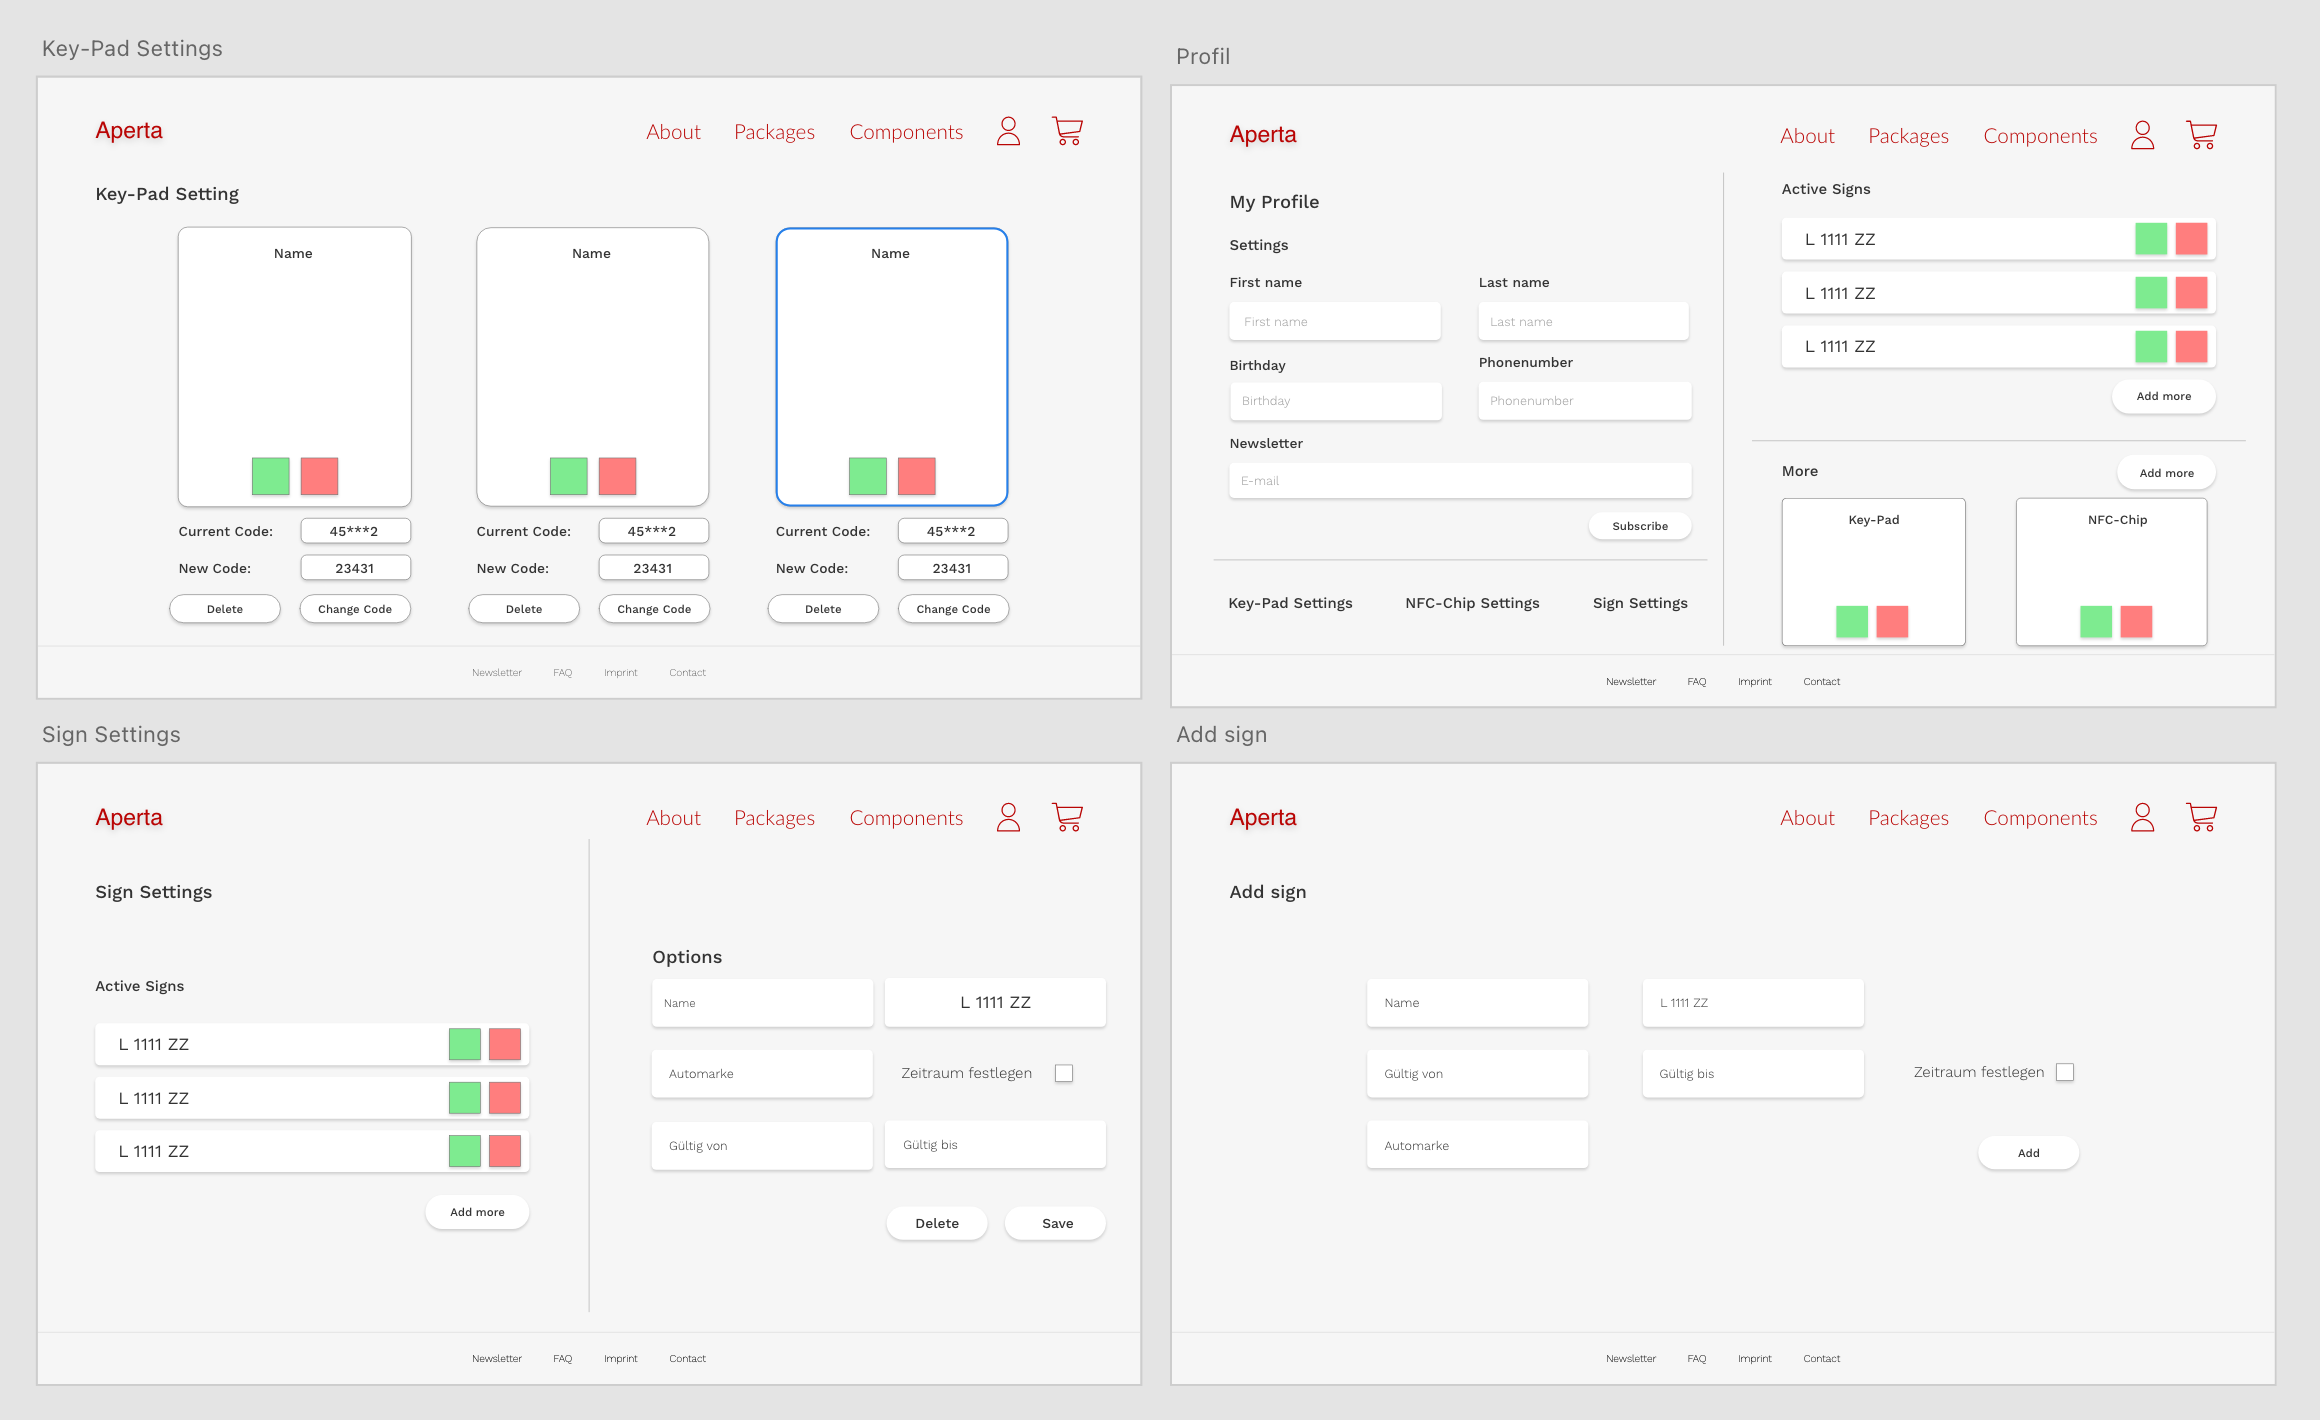
\includegraphics[width=0.6\textwidth]{pics/DashboardPrototyp.png}
    \caption{Prototyp des Dashboards}
  \end{figure}
  \begin{figure}[H]
    \centering
    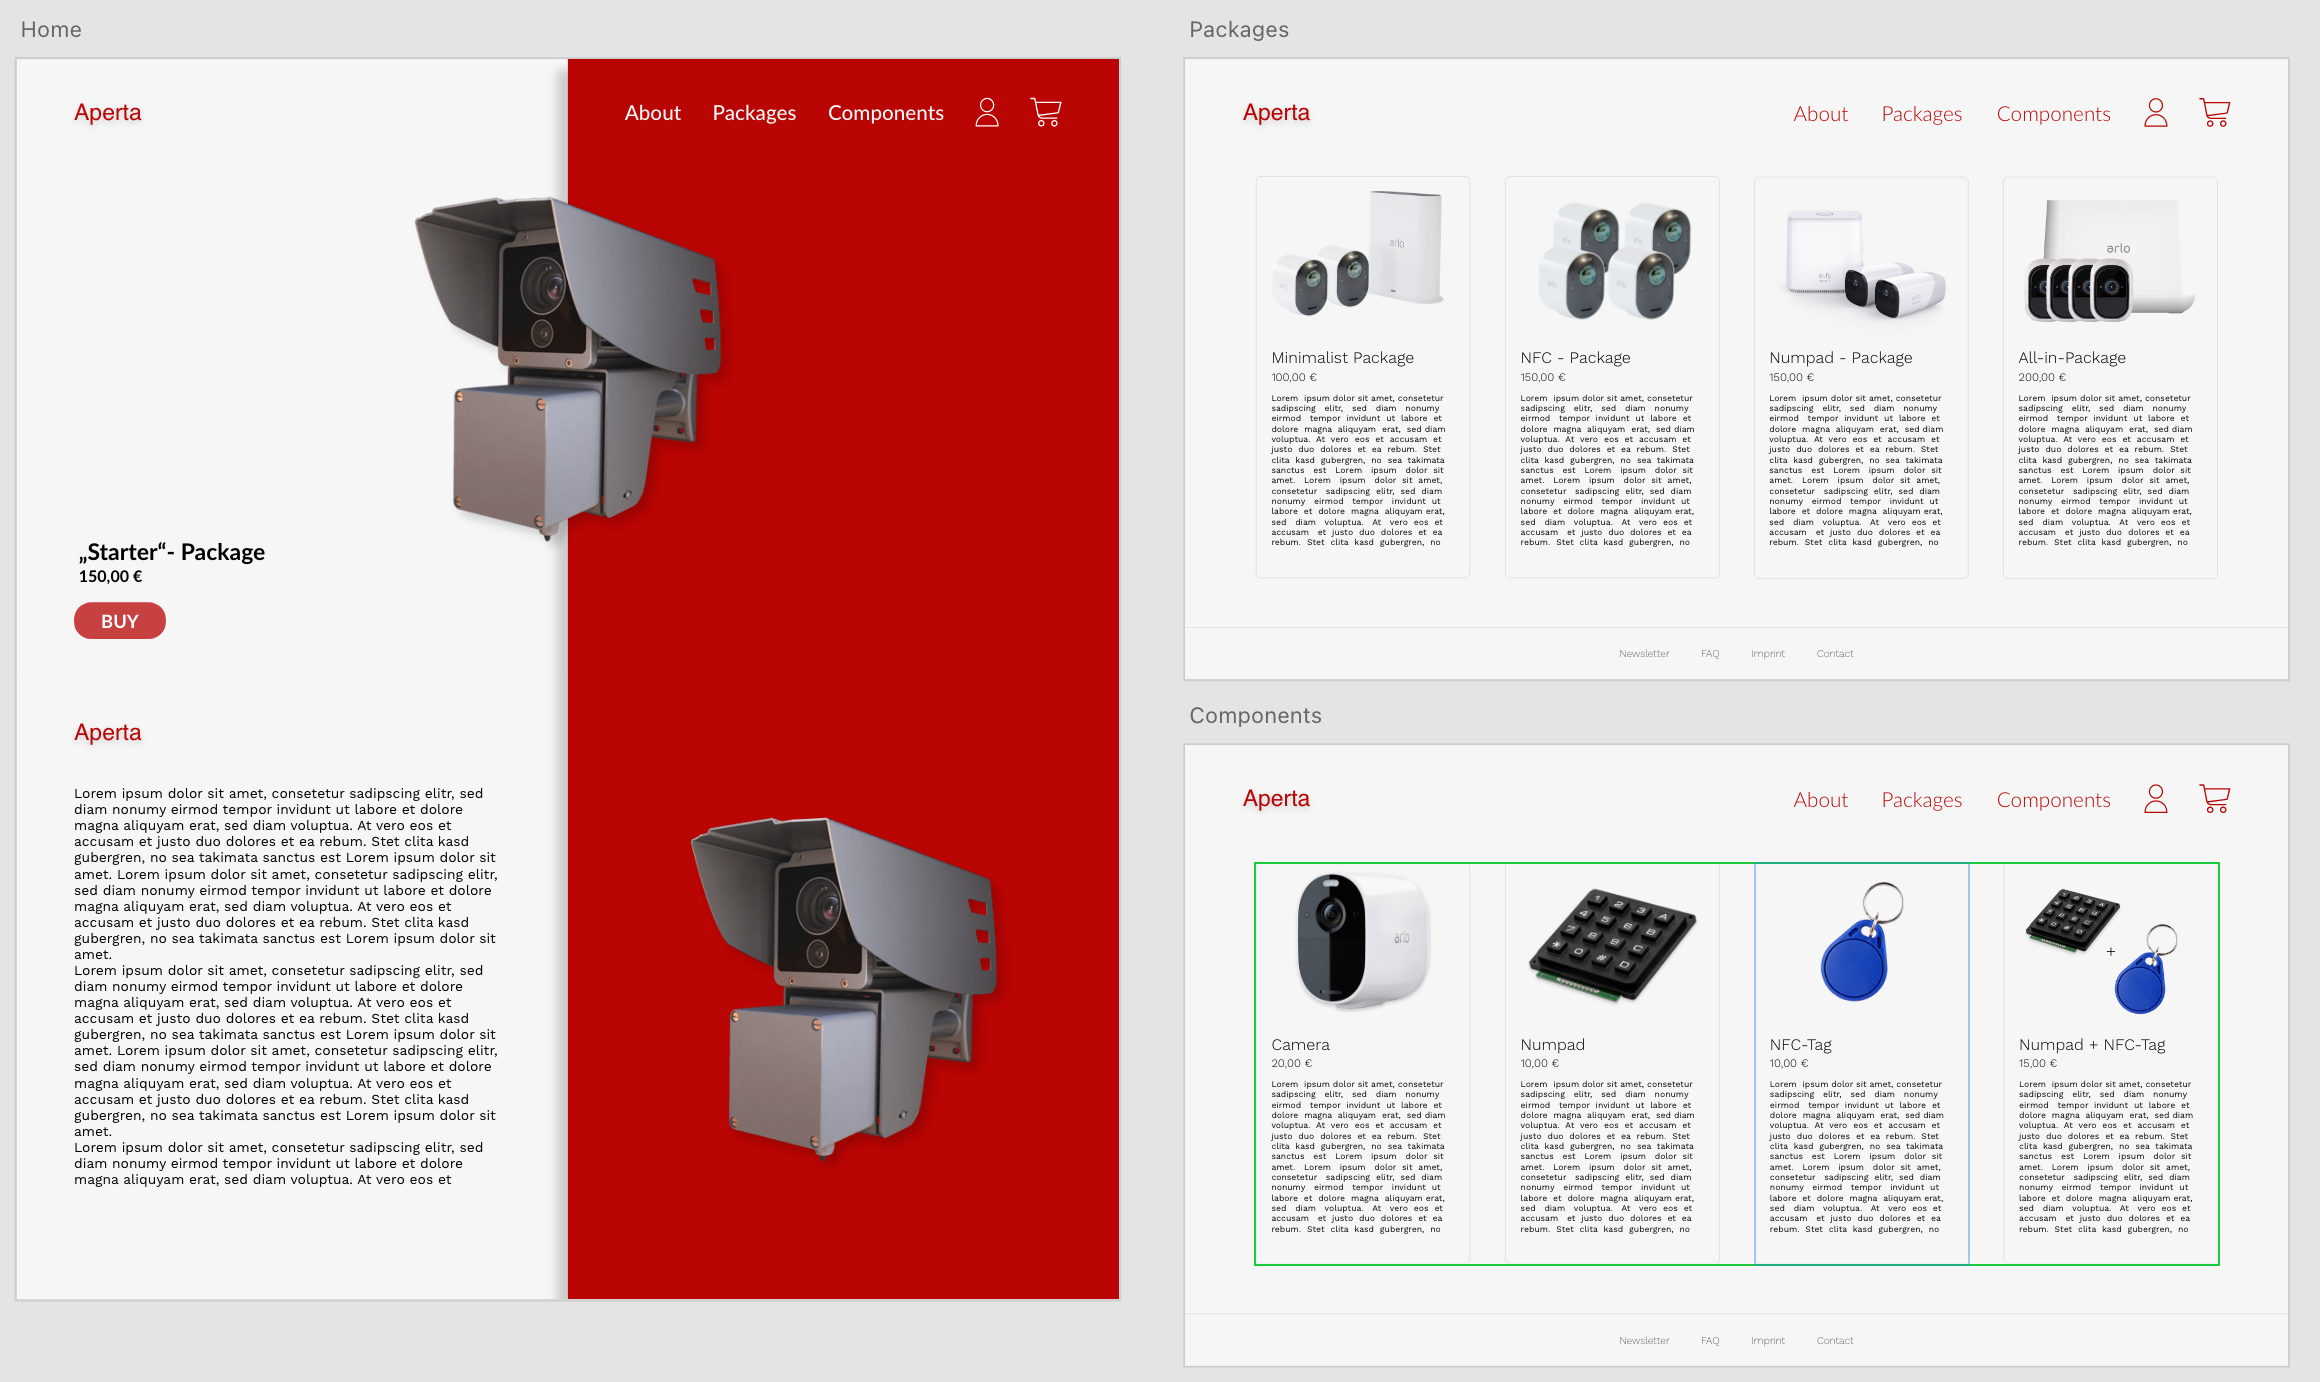
\includegraphics[width=0.6\textwidth]{pics/ShopPrototyp.png}
    \caption{Prototyp des Onlineshops}
  \end{figure}
  \newpage

Nach den Sommerferien 2021 wurden erste Teile, sowohl im Frontend als auch im Backend implementiert. Anfang November war das Design für die Profilseite und den Webshop fertig. Am Raspberry Pi hat die Kennzeichenerkennung bereits funktioniert und auch die Kommunikation mit der Datenbank wurde umgesetzt. Die Ergebnisse wurden unserem Betreuer Professor Aberger präsentiert.

In der nachfolgenden Zeit wurde das Projekt immer weiter vorangetrieben.  Anfang des Jahres 2022 war das Backend fertig implementiert und die Abfragen der Datenbank konnten im Profil verwaltet werden. Der Webshop war fertig, es fehlten nur noch ein paar Kleinigkeiten, die bis zum Ende fertig programmiert wurden. 

Der Fortschritt wurde erneut präsentiert und der Raspberry Pi konnte das Öffnen der Garage simulieren. Die Kennzeichenerkennung funktionierte, Codes konnten über das Nummernfeld eingegeben und NFC Chips gelesen werden. Auch der Webshop und das Profilmanagement hatten seine Funktion erfüllt. Die restliche Zeit wurde genutzt, um den schriftlichen Teil der Diplomarbeit fertigzustellen. 

\begin{figure}[H]
    \centering
    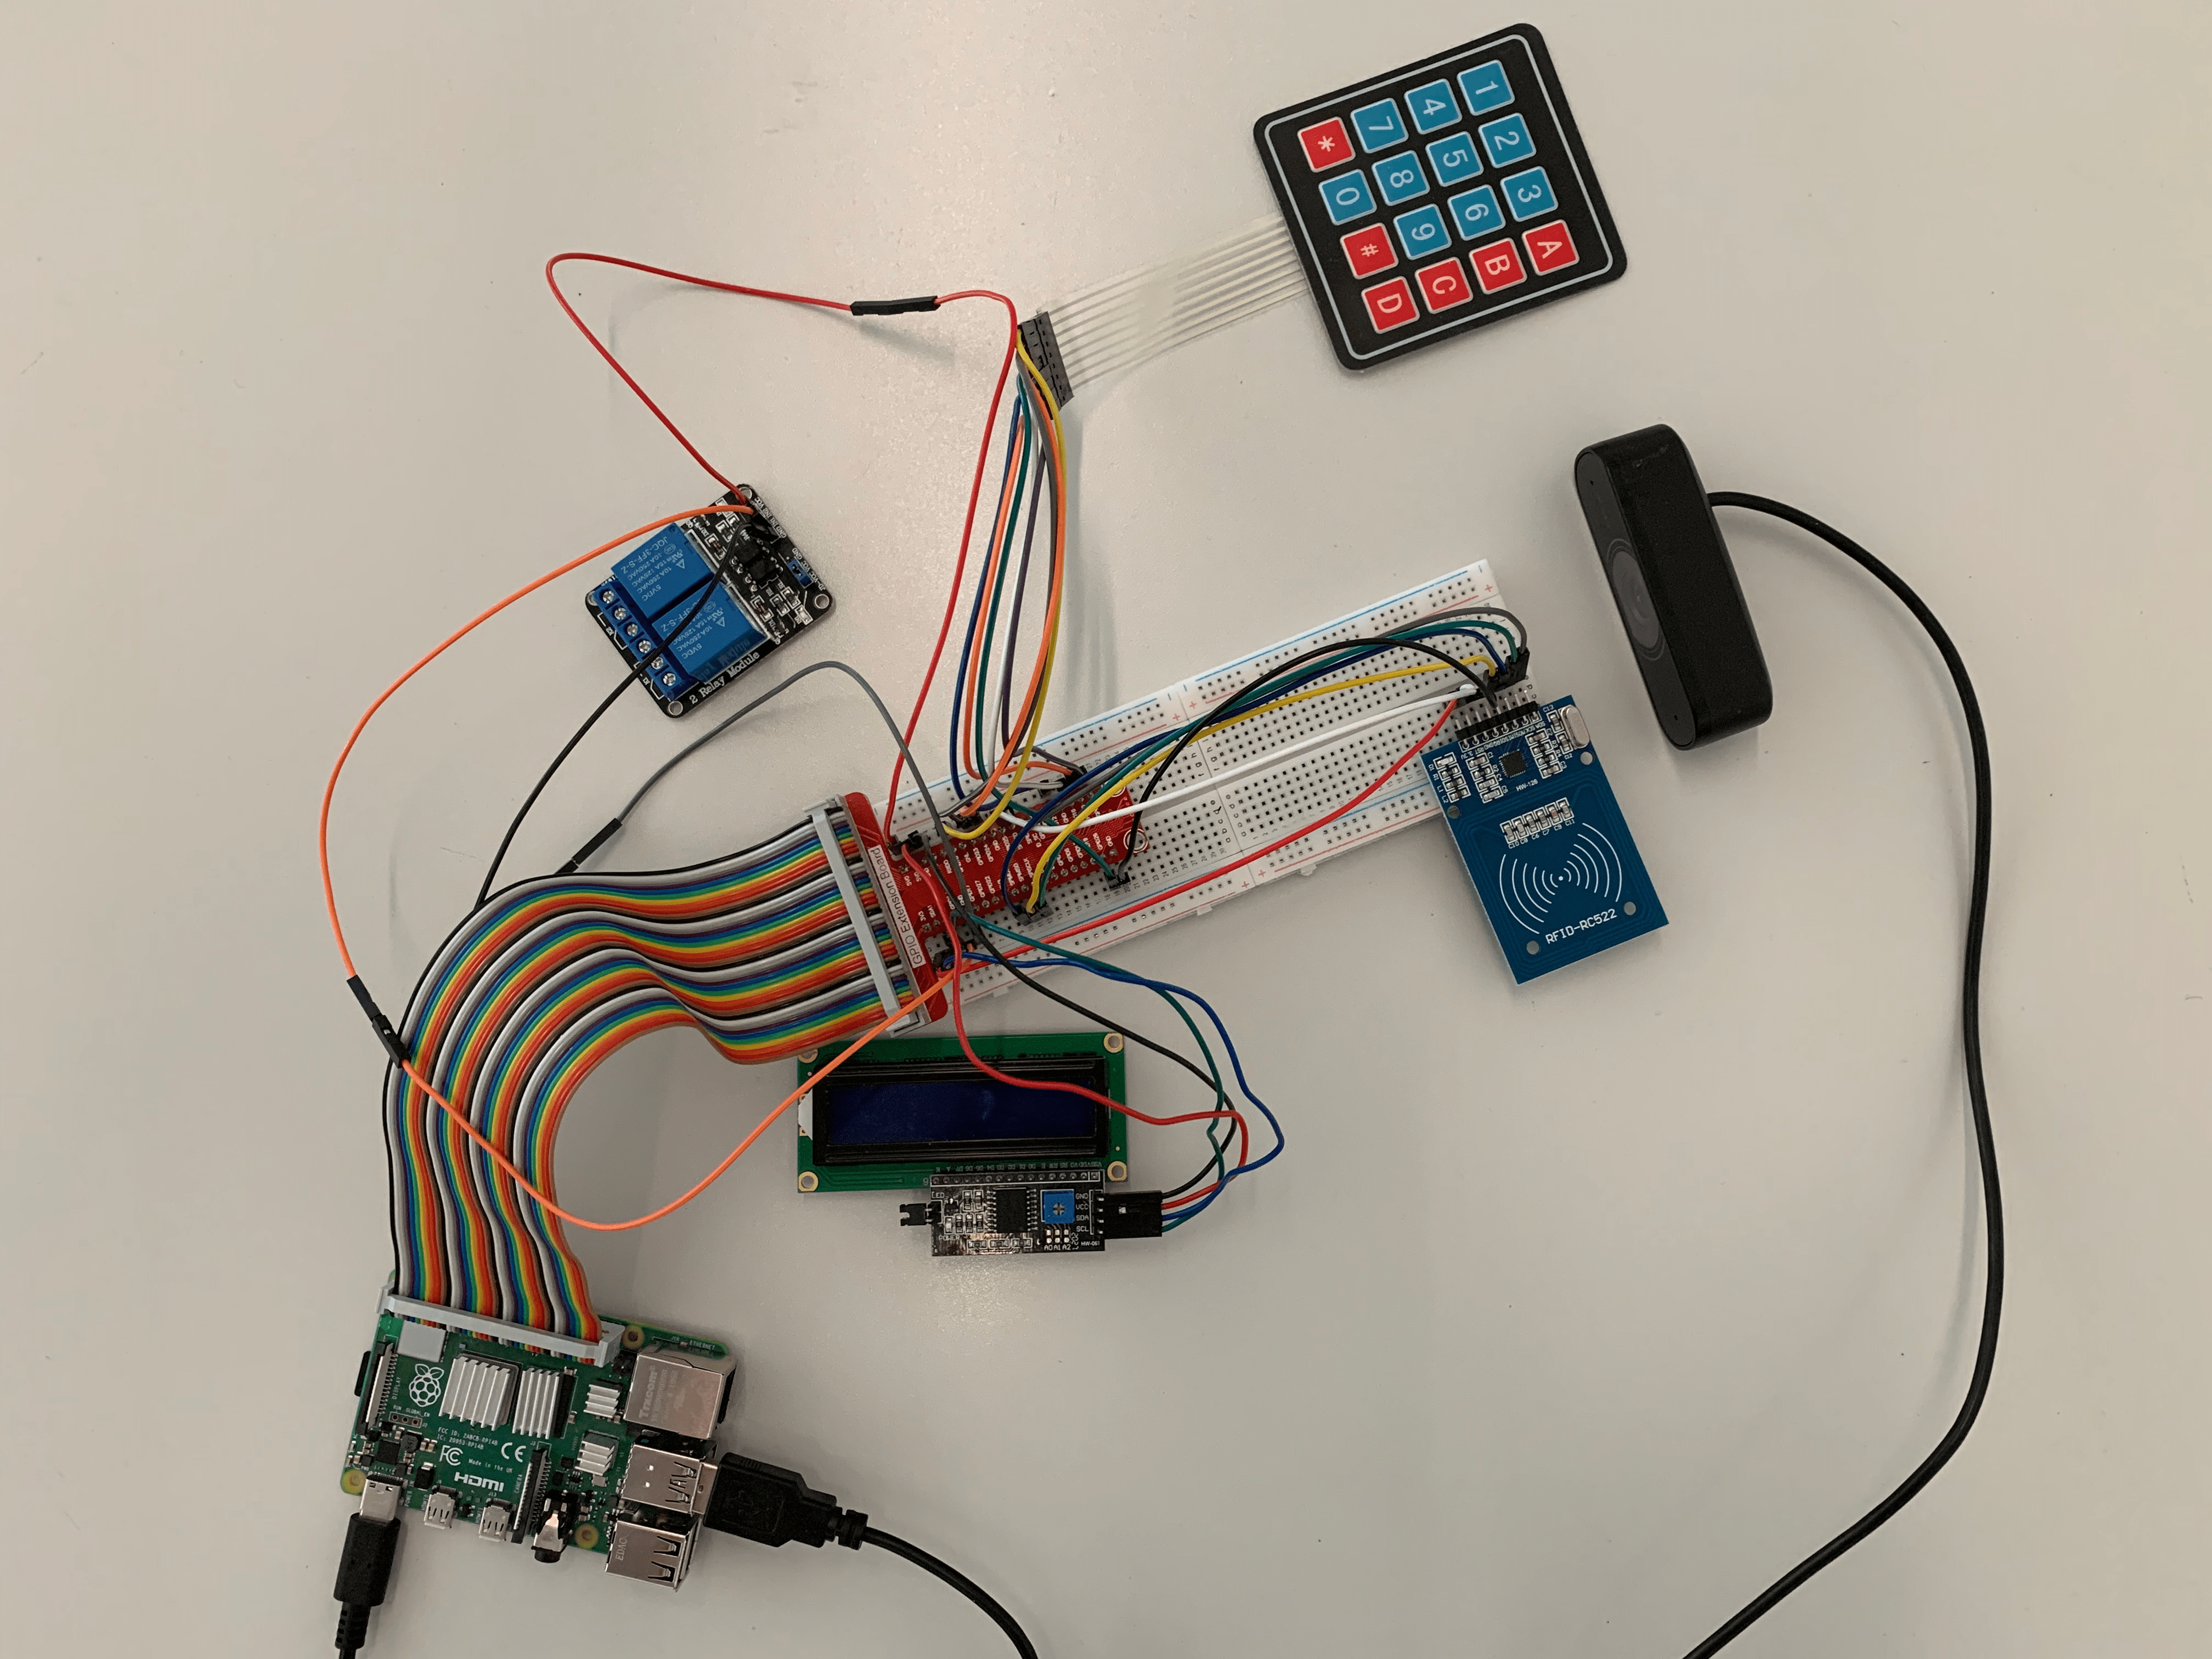
\includegraphics[width=0.6\textwidth]{pics/Aufbau.png}
    \caption{Aufbau der APERTA-Hardware}
  \end{figure}


\section{Erkenntnisse von Benjamin Golic}
\setauthor{Benjamin Golic}
Obwohl wir bereits im SEW- beziehungsweise ITP-Unterricht etwas größere Projekte durchgeführt haben, war dieses ganz anders. Trotz vieler unerwarteter und schwer lösbarer Fehler, konnte das Projekt zu ende entwickelt werden. 

Im Vergleich zu bisherigen Programmierprojekten hat mir die Zusammenarbeit bei diesem am meisten Freude bereitet. Wir konnten uns gegenseitig motivieren und haben uns auch gegenseitig geholfen, als jemand wo nicht mehr weitergekommen ist. 

Da wir Angular im SEW-Unterricht gelernt haben und ich kein so großer Freund davon bin, habe ich mich für React bei diesem Projekt entschieden. Der Umgang mit dieser Library gefiel mir so gut, dass ich mir vorstellen könnte, mich darauf für das spätere Berufsleben zu spezialisieren. 

\section{Erkenntnisse von David Hauser}
\setauthor{David Hauser}
Die Umsetzung des Projektes war nicht gerade einfach. Ich bin an einigen Punkten an meine Grenzen gestoßen. Dennoch hat mir die Zusammenarbeit mit meinen Kollegen viel Freude bereitet. Die Kommunikation mit ihnen ist immer reibungslos verlaufen und wir haben uns gegenseitig unterstützt, wo es nur möglich war.
Durch die Umsetzung mittels Angular konnte ich mein Wissen noch mehr vertiefen und festigen. Das Entwickeln mit einer bekannten Programmiersprache hat mir das Projekt sehr vereinfacht. Trotzdem waren einige Dinge für mich neu.
Der Beruf als Programmierer wird nicht mein zukünftiger werden. Das Programmieren hat mir teilweise sehr viele Nerven gekostet. Trotzdem hat das Team die Aufgaben gut erfüllt und die Zusammenarbeit war, wie erwähnt, sehr gut.

\section{Erkenntnisse von Simon Koll}
\setauthor{Simon Koll}

Das Projekt nahm immer mehr Substanz an, je weiter die Entwicklung fortschritt. Es kamen neue Ideen hinzu, die Anfangs noch gar nicht im Raum standen. Die Erkenntnisse und Inhalte des ITP-, INSY- sowie SEW-Unterrichts haben mich in der Entwicklung sehr unterstützt, da ich teilweise auf bereits vorhandenes Wissen aufbauen konnte. Gleichzeitig war es eine angemessene Aufgabe, die mich genug forderte, um die Motivation hoch zu halten. \\
Die Zusammenarbeit im Team ist eine der wichtigsten Erfahrungen, die ich in der Laufbahn der HTL bekommen habe. Es zeigt, wie wichtig die Kommunikation zwischen den Teammitgliedern ist und wie man sich gegenseitig motivieren kann.\\
Ich habe viele meiner bereits vorhandenen Kenntnisse vertiefen können, jedoch auch viel Neues über Bibliotheken wie OpenCV und Tesseract gelernt. Mit bereits bekannten und vertrauten Programmiersprachen zu arbeiten erleichterte die Entwicklung ungemein, da man bei Fehlermeldungen leichter erkennt, wo das Problem liegt und wie man es lösen kann.\\
Ich habe jedoch auch gelernt, dass ich in meiner Zukunft den Berufsweg eines Entwicklers vorraussichtlich nicht einschlagen werde, da diese Arbeit mich an manchen Punkten beinahe zur Verzweiflung brachte.
Zusammenfassend bin ich mit dem Ergebnis sowie der Leistung des Teams sehr zufrieden. 